\documentclass[sigconf]{acmart}
\setcopyright{none}
\settopmatter{printacmref=true}
\renewcommand\footnotetextcopyrightpermission[1]{}
\acmConference[ROSS '26]{15th International Workshop on Runtime and Operating Systems for Supercomputers}{November 15, 2026}{Chicago, IL, USA}
\acmBooktitle{15th International Workshop on Runtime and Operating Systems for Supercomputers (ROSS '26), November 15, 2026, Chicago, IL, USA}
\acmYear{2026}
\copyrightyear{2026}
\acmDOI{}
\acmISBN{}
\usepackage{booktabs}
\usepackage{tabularx}
\usepackage{array}
\usepackage{fancyvrb}
\usepackage{graphicx}
\urlstyle{same}
\providecommand{\tightlist}{\setlength{\itemsep}{0pt}\setlength{\parskip}{0pt}}
\setlength{\emergencystretch}{2em}

\title{Guarding HEFT-Style Placement against MSI-Induced Locality Conflicts in Multi-GPU Task Graphs}

% ROSS is single-blind. Final output must contain complete author metadata.
\author{Author Information Required}
\affiliation{\institution{Affiliation Required}\city{City Required}\country{Country Required}}
\email{email-required@example.invalid}

\begin{document}
\raggedbottom
\begin{abstract}
The HEFT-style device selector in CUDASTF accounts for communication that delays the current task, yet a favorable read--write placement can move the unique valid version of an object and induce larger successor traffic under the runtime's software MSI-style residency bookkeeping. We formalize this placement--residency conflict and its \emph{prefix-admissible} subclass, then introduce \textbf{prefix-safe copy-aware placement}: a lower-copy alternative is eligible only when it preserves the modeled finish of already committed placement decisions, up to a \(10^{-6}\) ms tolerance. The method predicts no unscheduled suffix, does not alter the runtime-supplied task order, and deliberately leaves non-admissible conflicts unchanged.

A qualified 75-run matrix covers five workloads on one 8-GPU NVIDIA L4 node and compares the runtime's HEFT-style baseline (H), prefix-safe placement (P), and exact gate removal (N). On the two workloads where P changes placement and reduces modeled copy, Cholesky and LU, it reduces modeled copy by 85.8\% and 38.8\% and improves latency over H by 1.405x and 1.173x. H, P, and N produce identical placement digests and copy totals on FDTD, CG, and MiniWeather; their observed timing ratios therefore cannot be attributed to locality decisions and instead bound scheduler-path, run-order, and system variation. Exact gate removal is 1.087x faster than P on Cholesky, exposing conservative gate cost, whereas P is 1.208x faster than N on LU despite N removing more copy, exposing harmful over-optimization. Eleven of fifteen workload--scheduler group medians miss our predeclared 5\% scheduler-share target, a prototype limitation. A separate controlled fixed-successor trace confirms the motivating migrate--return mechanism but is not used as performance evidence.

\end{abstract}
\ccsdesc[500]{Computer systems organization~Heterogeneous (hybrid) systems}
\ccsdesc[500]{Software and its engineering~Runtime environments}
\ccsdesc[300]{Theory of computation~Scheduling algorithms}
\keywords{multi-GPU task graphs, HEFT, data locality, runtime scheduling, copy traffic}
\maketitle

\section{Introduction}\label{introduction}

Online heterogeneous schedulers must decide where to execute a task before the rest of a dynamic graph has necessarily become runnable. The CUDASTF fork studied here uses a \emph{HEFT-style current-task device selector}: for the runtime-supplied next task, it estimates each device's earliest finish time (EFT), including current-input availability, and chooses the minimum. Unlike canonical offline HEFT, it does not compute an upward-rank task order. This distinction matters: our contribution refines device placement, not DAG ordering.

The local objective is nevertheless incomplete when placement changes data state. CUDASTF's \emph{software} MSI-style bookkeeping leaves a new read--write version Modified on the selected GPU and invalidates stale copies; it is not a claim about a hardware cache-coherence protocol. A placement that wins a fraction of a millisecond for the current task can consequently move a large mutable version away from the GPU where a later task consumes it. The later task either copies the version back or follows it and moves other inputs. In both cases the locally best EFT decision can initiate a residency cascade whose traffic is larger than the immediate gain. We use ``HEFT--MSI conflict'' as shorthand for this interaction between the runtime's HEFT-style selector and its software residency model.

This paper asks a general systems question: can an online scheduler exploit residency-aware copy savings without paying arbitrary delay in the work already committed? Our answer is a prefix-bounded refinement. We first retain HEFT's device as a baseline. We then consider devices that reduce modeled current-input copy and admit one only if its finish fits the baseline's current-prefix finish bound up to numerical tolerance. The rule is benchmark-independent: it applies to ordinary tasks and does not require a special mutable-chain label. Its opportunity is nevertheless a strict subclass of all HEFT--MSI conflicts: the current ready frontier must hide the alternative's HEFT-relative delay. The condition says nothing about the makespan of the unscheduled suffix.

As a diagnostic, we also ask whether the motivating migrate--return pattern can be identified directly in a controlled case. A narrow successor-aware locality certificate (SALC) compares a one-hop avoided output-copy lower bound against the producer's HEFT-relative EFT damage when the successor has an explicit fixed device. This trace validates the motivating mechanism; SALC is not presented as a second general scheduler or as natural-CG performance.

Our contributions are:

\begin{enumerate}
\def\labelenumi{\arabic{enumi}.}
\tightlist
\item
  We formalize a legal migrate--return counterexample between CUDASTF's HEFT-style current-task selector and its software MSI-style residency transitions, and distinguish the prefix-admissible subclass that the main method can change.
\item
  We define and implement a translation-invariant, prefix-safe copy-aware refinement, together with an exact gate-removal ablation. The gate enforces an explicit current-prefix admission contract while optimizing a secondary copy-and-queue score; it is not claimed to repair every HEFT--MSI conflict.
\item
  We evaluate opportunity, response, and gate risk separately. A qualified 75-run matrix identifies two effective different-placement cases, three identical-placement drift controls, and opposite gate-ablation outcomes; a controlled fixed-successor trace supplies diagnostic mechanism evidence.
\end{enumerate}

The resulting claim is deliberately smaller than ``automatic chain discovery'' but broader than a policy for two named benchmarks. Prefix safety is a general admission rule for the prefix-admissible subclass of placement--residency conflicts; the fixed-successor trace only certifies one graph-visible edge pattern. Neither result proves a suffix or global makespan improvement, and a benchmark-independent rule does not imply universal applicability or speedup.

\section{System Model and HEFT--MSI Conflict}\label{system-model-and-heftmsi-conflict}

\subsection{Online task and residency model}\label{online-task-and-residency-model}

Let \(G=(V,E)\) be a task DAG and \(D=\{0,\ldots,m-1\}\) the GPU set. Task \(v\) has predicted compute time \(p_v>0\). A logical data object \(x\) has modeled copy time

\[
c_x = \frac{\operatorname{bytes}(x)}{B},
\]

where \(B\) is the scheduler's explicit copy-bandwidth parameter. At scheduling step \(k\), \(L_k(d)\) is GPU \(d\)'s modeled ready time and \(M_k(x,d)\in\{M,S,I\}\) is the scheduler's software Modified/Shared/Invalid residency state.

For current task \(v\), let \(A_k(v,d)\) be the latest availability time among its read and read--write inputs on \(d\). A local Modified or Shared instance incurs no transfer; otherwise availability includes a copy from a valid instance. CUDASTF's current HEFT estimate is

\[
F_k(v,d) = \max\{L_k(d), A_k(v,d)\} + p_v,
\qquad
b = \arg\min_{d\in D} F_k(v,d),
\]

with a deterministic tie order. We call \(b\) the \textbf{HEFT baseline device}. After a write-like access on \(d\), the scheduler's MSI transition makes the new version valid at \(d\) and invalidates conflicting copies elsewhere.

Here ``HEFT'' denotes this CUDASTF fork's HEFT-style current-task device selector; the runtime supplies task order rather than recomputing the offline upward-rank order of canonical HEFT. Equal-EFT candidates are resolved by lower device ID.

This formulation also explains why the earlier copy-gain-plus-penalty idea can work even though HEFT already models communication. HEFT folds current input readiness into a \textbf{maximum} before adding compute time, whereas the secondary copy quantity \(K(d)\) below \textbf{sums} modeled transfers. A busy device or one late dependency can dominate \(F_k\) and hide several other transfers: two devices can have the same current-prefix finish while moving very different total bytes. Copy gain exposes that hidden locality slack; the prefix gate prevents the scheduler from buying lower traffic by extending the finish frontier that HEFT has already established. The method is therefore a secondary refinement of HEFT, not a claim that HEFT ignores communication.

The transfer quantities reported in this paper require precise language. \textbf{Modeled copy bytes/time} are computed by the scheduler's MSI and bandwidth model. \textbf{Runtime-issued GPU-peer transfers} are data-interface copies that CUDASTF actually requests between distinct GPU endpoints. They are not CUPTI transactions, link utilization, or physical PCIe/NVLink bus traffic.

\subsection{Conflict definition}\label{conflict-definition}

Let \(\Phi_k(v,d)\) denote the future data-movement penalty induced by placing \(v\) on \(d\). This is a conceptual suffix quantity, not something our main method computes. A HEFT--MSI locality conflict exists for devices \(g,h\) when

\[
F_k(v,g) < F_k(v,h)
\]

but

\[
\Phi_k(v,g)-\Phi_k(v,h)
  > F_k(v,h)-F_k(v,g).
\]

Thus the ordering of \(g\) and \(h\) is reversed under \(F_k+\Phi_k\). When \(D=\{g,h\}\), as in the construction below, their global minimizers differ; with more devices, the definition asserts only this pairwise reversal.

A two-GPU construction establishes existence. Let a mutable object \(x\) be valid on GPU 1 and invalid on GPU 0, with copy time \(C\). Set GPU loads to \(L(0)=0\) and \(L(1)=C+\epsilon\), where \(0<\epsilon<C\). A read--write task \(v\) finishes at \(C+p_v\) on GPU 0 and at \(C+\epsilon+p_v\) on GPU 1, so HEFT moves \(x\) to GPU 0 for an \(\epsilon\) advantage. Now give successor \(u\) another large input that fixes its preferred execution at GPU 1. Under HEFT, \(u\) copies the new version of \(x\) back at cost \(C\); if \(v\) had stayed on GPU 1, that copy would be absent. Thus the construction proves one object-sized return transfer, whose modeled time is \(C\). If \(u\) lies on the serial dependency path, no intervening task overwrites \(x\), and the return copy is not completely hidden by other waiting, the suffix completion additionally loses \(C-\epsilon>0\).

This is an existential statement. It does not imply that HEFT usually fails, that every read--write task belongs to a harmful chain, or that any local correction improves the full DAG. In fact, the two-GPU construction is intentionally stronger than the scope of the prefix-safe method: as shown below, its alternative extends the current prefix and is rejected.

\section{Bounded Locality Refinements}\label{bounded-locality-refinements}

\subsection{Prefix-safe copy-aware HEFT}\label{prefix-safe-copy-aware-heft}

For the current task, let \(K(d)\) be the sum of modeled transfer times for its read and read--write inputs on device \(d\). Let \(T(d)=\max\{L_k(d),A_k(v,d)\}\) and define the modeled queue delay

\[
Q(d)=\max\{0,T(d)-A_k(v,d)\}.
\]

We first compute the HEFT baseline \(b\), breaking equal EFTs by lower device ID. Let

\[
R = \max_{d\in D} L_k(d)
\]

be the current ready-time frontier (the implementation's current-system-finish accumulator, defensively recomputed from all candidate device-ready times), and define the baseline and candidate prefix finishes

\[
P_b = \max\{R,F(b)\}, \qquad P(d)=\max\{R,F(d)\}.
\]

The prefix gate admits \(d\ne b\) only if

\[
P(d) \le P_b + \varepsilon_p.
\]

We call a HEFT--MSI conflict \textbf{prefix-admissible} for candidate \(d\) when it has positive modeled current-input copy saving, satisfies the frozen copy-gain threshold, and passes this prefix gate. This definition exposes rather than hides the method boundary. In the two-GPU construction above, \(R=C+\epsilon\) (assuming no larger prior frontier), and the owner-preserving alternative has

\[
P(1)-P_b
= C+\epsilon+p_v-\max\{C+\epsilon,C+p_v\}
= \min\{\epsilon,p_v\}>0.
\]

It is therefore rejected for a tolerance smaller than both \(\epsilon\) and \(p_v\). The admissible subclass is nevertheless nonempty. Add an independently busy GPU 2 with ready time \(H\ge C+\epsilon+p_v\), while keeping its own candidate finish larger than those of GPUs 0 and 1. GPU 0 remains HEFT's device for \(v\), but the global ready frontier becomes \(R=H\), so \(P(0)=P(1)=H\). Staying with the valid owner on GPU 1 then passes the gate, has \(K(1)=0<K(0)=C\), and avoids the modeled return transfer without increasing the current prefix. Cholesky and LU provide the evaluated, non-synthetic observations of this hidden-slack opportunity.

An alternative may therefore have a later per-task EFT than HEFT when that difference is hidden under the already established ready frontier, but it may increase the modeled finish of the current scheduling prefix by at most the numerical tolerance \(\varepsilon_p\). Shifting every modeled timestamp---including availability, ready, and finish times---by the same constant changes neither this decision nor the queue-delay terms, avoiding a sensitivity of gates normalized by absolute EFT.

\textbf{Modeled current-prefix contract.} If candidate \(d\) passes the gate above, replacing \(b\) by \(d\) increases the scheduler's current prefix-finish quantity by at most \(\varepsilon_p\). This follows directly from the acceptance predicate \(P(d)\le P_b+\varepsilon_p\); it is an enforceable contract, not a theorem about the suffix. Adding the same constant to every ready and finish time leaves both sides unchanged, so the predicate is time-shift invariant. The implementation fixes \(\varepsilon_p=10^{-6}\) ms. The contract concerns the model's scalar \(\max\{R,F\}\); it does not preserve the current task's EFT, the unscheduled suffix, or observed wall time. Here ``prefix'' means placement decisions already committed, not a predicted critical-path prefix.

Among prefix-safe alternatives, we retain the existing copy-aware selectivity. Define

\[
G_K(d)=\frac{K(b)-K(d)}{\max\{K_{\min},K(b)\}},
\qquad
G_Q(d)=\frac{Q(b)-Q(d)}{\max\{Q_{\min},Q(b)\}}.
\]

The candidate must have a strictly positive copy saving and satisfy \(G_K(d)\ge\tau\). Let \(n_v\) be dependency count, \(B_v\) the bytes of read/read--write inputs, \(p_v\) the predicted task time in ms, and \(\operatorname{clip}(z)=\min\{1,\max\{0,z\}\}\). Define

\[
\begin{aligned}
c_p&=\operatorname{clip}\!\left(\frac{\ln(1+p_v)}{\ln 501}\right),
&c_n&=\operatorname{clip}\!\left(\frac{n_v}{16}\right),\\
c_B&=\operatorname{clip}\!\left(\frac{\ln(1+B_v)}{\ln(1+2^{30})}\right),
&c(v)&=\operatorname{clip}(0.55c_p+0.30c_n+0.15c_B).
\end{aligned}
\]

In the frozen configuration, \(K_{\min}=Q_{\min}=0.001\) ms, \(\tau=0.25\) when \(c(v)>0.60\) and \(0.15\) otherwise, and \(\lambda_Q=0.35\). These inherited values are shared by every benchmark, were frozen before the repeated confirmation, and are not claimed optimal. Eligible alternatives are ranked by

\[
S(d)=G_K(d)+\lambda_Q\max\{0,G_Q(d)\},
\]

then by lower EFT and lower device ID under a score tie. The selected device is HEFT when no candidate passes both gates.

\begin{Verbatim}[fontsize=\scriptsize]
PREFIX-SAFE-COPY(task v, candidates D)
    b <- runtime HEFT-style candidate
    R <- max device ready time
    P_b <- max(R, F(b))
    eligible <- empty
    for d in D, d != b:
        if candidate fields are not finite: continue
        copy_saving <- K(b) - K(d)
        copy_gain <- copy_saving / max(K_min, K(b))
        if copy_saving <= eps or copy_gain < tau(v): continue
        if F(d) > P_b + eps_prefix: continue
        queue_gain <- (Q(b) - Q(d)) / max(Q_min, Q(b))
        score <- copy_gain + lambda_Q * max(0, queue_gain)
        add (d, score) to eligible
    if eligible is empty: return b
    return highest score, then lower EFT, then lower device ID
\end{Verbatim}

The method records accepted copy saving, HEFT-relative EFT damage, and prefix damage. Verification requires aggregate prefix damage to be zero within numerical tolerance. The broad mode is our main method. A one-read--write/unique-owner restriction was also implemented, but every task in the studied Cholesky and LU DAGs satisfied that scope, and the restricted and broad variants produced identical placements. The scope is therefore not evidence of chain detection.

For controlled mechanism isolation, the source-matched \texttt{no-prefix} ablation retains the same HEFT-style baseline, candidate set, copy and queue gains, thresholds, score, and tie breaks, but disables only the prefix admission rule. It consequently has no prefix contract. This exact removal distinguishes the gate's effect from the earlier conventional relative-EFT comparator, which changes the timing rule itself.

\subsection{Diagnostic fixed-successor certificate}\label{fixed-successor-salc-companion}

Prefix safety cannot accept a device whose current EFT extends \(P_b\), even when one known future copy is much larger. SALC addresses only a graph-visible version of that case.

For producer \(v\), SALC identifies write-like output symbols read by direct successors. If successor \(u\) is explicitly fixed to GPU \(a(u)\), that GPU is an authoritative anchor. For a hypothetical producer device \(d\), a conservative one-hop modeled copy quantity is

\[
\Phi_1(d)=
\sum_{(x,a)\in U}
\mathbf{1}[d\ne a]\frac{\operatorname{bytes}(x)}{B},
\]

where \(U\) deduplicates output-symbol/anchor pairs. For HEFT baseline \(b\) and alternative \(d\), SALC computes

\[
G_{\mathrm{future}}(d)=\Phi_1(b)-\Phi_1(d),
\qquad
\Delta_F(d)=\max\{0,F(d)-F(b)\},
\]

and accepts only when

\[
C_{\mathrm{SALC}}(d)
=G_{\mathrm{future}}(d)-\Delta_F(d)
> \mu,
\]

for margin \(\mu\) (zero in the controlled certificate). SALC selects the positive candidate with the largest certificate, breaking ties by EFT.

The inequality is a certificate only when the producer creates the unique relevant version, the fixed successor reads that same version, and no intervening task overwrites it. It certifies a modeled one-hop edge risk, not actual saved link time, critical-path delay, suffix speedup, or global makespan. Although the implementation can form a shadow anchor for non-fixed successors, the positive evidence here is specifically the authoritative fixed-successor case.

\section{Controlled Mechanism Diagnostic}\label{controlled-cg-derived-chain-certificate}

We constructed a controlled residual-audit path inside CG to realize the formal conflict without presenting it as natural CG performance. The setup initializes a 128 MiB target version on GPU 0. Under wrappers pinned to canonically identical calibration content and strict task keys, HEFT places read--write task 46 (\texttt{cg\_axpy}) on GPU 1; an independent runtime-load attestation was unavailable. A direct \texttt{cg\_dot} successor is fixed to GPU 0, so task 48 returns the produced data; five later fixed reads repeat that direction.

The corrected fixed-anchor SALC implementation makes exactly one direct intervention: task 46 stays on GPU 0. Its one-copy future lower bound is 6.483948 ms, its HEFT-relative EFT damage is 0.474260 ms, and the certificate is therefore 6.009688 ms. Replaying the independently recorded HEFT decisions shows 28 final placement differences: the direct task plus 27 downstream cascade changes.

\begin{table*}[t]
\centering
\caption{Controlled CG-derived fixed-successor certificate.}\label{tab:controlled-cg-certificate}
\footnotesize
\setlength{\tabcolsep}{3pt}
\begin{tabularx}{\textwidth}{@{}>{\raggedright\arraybackslash}p{0.27\textwidth}>{\raggedright\arraybackslash}X>{\raggedright\arraybackslash}X@{}}
\toprule
Controlled trace property & HEFT & Fixed-successor SALC \\
\midrule
Direct residual interventions & 0 & 1 (task 46, GPU 1 -> GPU 0) \\
Modeled owner round trips & 1 & 0 \\
Target runtime-issued GPU-peer bytes & 939,524,096 & 0 \\
Total runtime-issued GPU-peer bytes & 2,684,355,048 & 480 \\
All runtime-issued transfer bytes & 4,563,403,232 & 939,524,592 \\
Relative residual correctness gap & PASS & 2.3954e-16 (PASS) \\
\bottomrule
\end{tabularx}
\end{table*}

The remaining 480 peer bytes under SALC are scalar traffic unrelated to the target. Target peer bytes fall by 100\%, total peer bytes by 99.99998\%, and all runtime-issued bytes by 79.41\%. The artifact verifier joins task/data identity with the fixed-successor interval and recomputes SALC's placement digest; runtime rows do not contain an independent data-version epoch, so attribution is explicitly conditional rather than overstated.

\begin{figure*}[t]
\centering
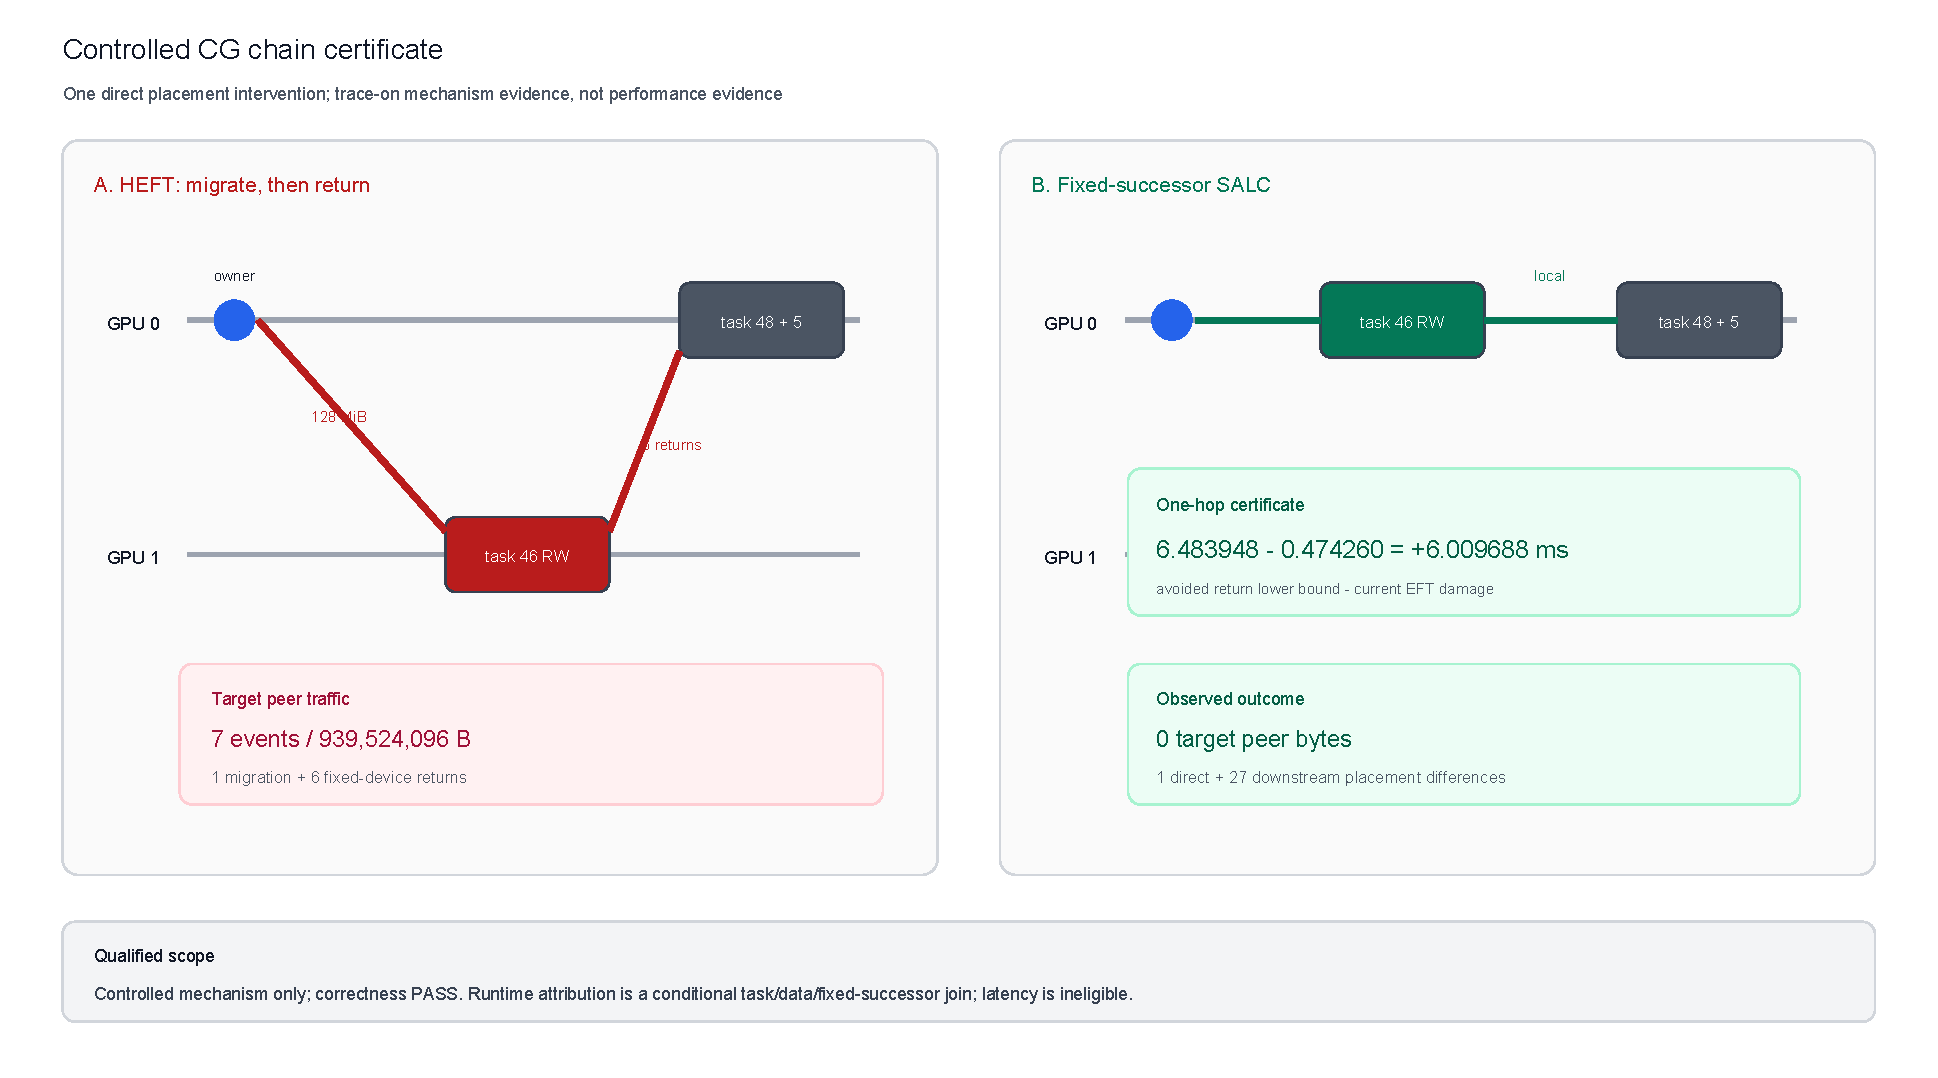
\includegraphics[width=\textwidth]{figures/controlled_cg_chain_certificate.pdf}
\Description{Controlled CG-derived migrate--return pattern and the fixed-successor SALC certificate. The figure summarizes trace-on, controlled mechanism evidence; its latency is not performance eligible and its task/data attribution is conditional.}
\caption{Controlled CG-derived migrate--return pattern and the fixed-successor SALC certificate. The figure summarizes trace-on, controlled mechanism evidence; its latency is not performance eligible and its task/data attribution is conditional.}
\end{figure*}

The observations are single, instrumented, and split across two pinned task wrappers. We therefore use no latency difference from this experiment; it establishes only an intervention-consistent decision-and-traffic certificate.

\section{Experimental Methodology and Evidence Discipline}\label{experimental-methodology-and-evidence-discipline}

\subsection{Platform, workloads, and schedulers}\label{platform-workloads-and-schedulers}

The primary problem-boundary matrix executed source \texttt{673f8c19\allowbreak{}d73280be\allowbreak{}02733b80\allowbreak{}6285339e\allowbreak{}e8699950} on one dual-NUMA Europa node with eight NVIDIA L4 GPUs (23,034 MiB each), driver 595.71.05, CUDA 12.4.131, GCC 13.3.0, CMake 4.3.4, CUDASTF 3.2.0.0, and a C++17 Release build. The historical strong-opportunity confirmation executed source \texttt{cfdd6d1f\allowbreak{}f8f1c45c\allowbreak{}8c9c0da6\allowbreak{}2a859452\allowbreak{}dce09b86} on the same platform. GPUs 0--3 and 4--7 form separate NUMA-local PCIe groups; cross-group traffic traverses the system interconnect. A nearby metadata snapshot identifies a dual-socket Intel Xeon Gold 6548N host, but its clock and persistence readings are not treated as steady-state attestations.

The scheduler uses one scalar 20.7 GB/s copy parameter, derived from a complete directed-pair microbenchmark with 20.726 GB/s median. It does not model the NODE/SYS pair distinction, contention, or copy/compute overlap. Robust task-cost calibration runs on GPU 0 and is then shared across the eight identical L4s.

\begin{table*}[t]
\centering
\caption{Workload configurations and validation contracts.}\label{tab:workloads}
\footnotesize
\setlength{\tabcolsep}{3pt}
\begin{tabularx}{\textwidth}{@{}>{\raggedright\arraybackslash}p{0.23\textwidth}>{\raggedright\arraybackslash}X>{\raggedright\arraybackslash}X>{\raggedright\arraybackslash}X>{\raggedright\arraybackslash}X@{}}
\toprule
Workload & Arguments & Precision & Submitted tasks & Structure and validation \\
\midrule
FDTD & \texttt{\detokenize{672 64 64 64}} & FP64 & 4,704 & 3-D electromagnetic stencil; finalized host \(E_z\) checksum and norms \\
Cholesky & \texttt{\detokenize{28672 256}} & FP64 & 240,464 & 112 x 112 tiled dense factorization; projected backward error and checksum \\
LU decomposition & \texttt{\detokenize{23552 256}} & FP64 & 263,810 & 92 x 92 tiled no-pivot factorization; projected residual and checksum \\
MiniWeather & \texttt{\detokenize{1536 2048 1536}} & FP64 & 55,296 & six independent finite-horizon regional RK3 chains; finalized changed-state checksum \\
Standard CG & \texttt{\detokenize{16777216 40 10}} & FP64 & 3,040 & 40 static contexts with bounded iterations and finalized checksum; one historical identity-control block is excluded \\
\bottomrule
\end{tabularx}
\end{table*}

Workload names do not define the method's scope. Table~\ref{tab:workloads} samples distinct problem conditions in the primary repeated matrix. Cholesky and LU expose substantial modeled-copy opportunity and different H/P/N placement digests. FDTD, CG, and MiniWeather produce identical H/P/N placement digests and modeled-copy totals, so they measure scheduler-path, fixed-order, and system timing variation rather than the effect of a locality decision. Standard CG also supplies prior identity-control and certificate evidence. The Cholesky and LU configurations were frozen after one-run exploration and are therefore mechanism-bearing cases, not an unbiased prevalence survey. We use them to test the response to prefix-admissible HEFT--MSI opportunities, not to claim that dense factorization is the method's target domain.

All repeated workloads set \path{CUDASTF_THESIS_DEFER_KERNEL_TASKS=1}: each DAG is fully materialized before \texttt{ctx.submit()}. Placement decisions remain sequential and irrevocable, and prefix-safe itself uses no successor prediction, but these experiments do not validate dynamic task arrival. Cholesky and LU record a CUDA start event immediately before DAG construction and a completion event after deferred submission finishes; the reported benchmark interval therefore spans graph construction, scheduling-induced gaps, and GPU execution, but excludes the subsequent correctness check.

The historical strong-opportunity matrix contains HEFT (H), prefix-safe (P), and exact no-prefix (N) on Cholesky and LU, in fixed H--P--N order for five repeats: \(2\times3\times5=30\) executions. H is also the runtime-default scheduler in this fork. P and N share the baseline, candidates, gains, thresholds, score, and tie breaks; N disables only prefix admission. Each benchmark performs a fresh robust single-GPU calibration prepass shared across the three variants. Calibration discards warm-up sample 0, retains samples 1--9, requires at least 7/9 within \(\max(25\%\text{ of median},0.005\text{ ms})\), and requires scaled MAD no greater than \(\max(10\%\text{ of median},0.005\text{ ms})\).

That performance-eligible block disables per-task \texttt{COPY\_TASK}, decision, comparator-shadow, and runtime-transfer tracing; only aggregate scheduler summaries remain enabled. All 30 executions pass the predeclared provenance, completeness, calibration, correctness, and deterministic placement/copy/checksum checks. Performance direction and the scheduler-share target are reported outcomes, not qualification criteria.

Our primary problem-boundary protocol is a separate current-source block over FDTD, standard CG, Cholesky, LU, and MiniWeather. It retains the same fixed H--P--N order and frozen scheduler parameters for five repeats, giving \(5\times3\times5=75\) executions; its timings are not pooled with the historical 30-run block. Each workload again performs one fresh GPU-0 calibration shared by its three variants. The estimator still discards reservation 0 and takes the median of reservations 1--9. The independently frozen \texttt{scalar\_microkernel\_v2} quality rule requires scaled MAD no greater than \(\max(10\%\text{ of median},f)\). It requires at least 6/9 samples within \(\max(25\%\text{ of median},f)\) only when the task footprint is at most 24 bytes and the median is below 0.050 ms, with \(f=0.025\) ms; every other task retains the 7/9 requirement and \(f=0.005\) ms. This structural exception handles repeatable same-GPU contention tails on launch-bound scalar kernels while preserving a two-thirds central majority and the independent MAD gate. The rule was fixed from raw calibration failures before any expanded-block performance result was read; raw samples, selected floors, inlier counts, and pass/fail decisions remain archived. All 75 executions pass fail-closed checks for matrix order and completeness, hardware identity, calibration freshness and quality, raw-log linkage, build and mechanism provenance, independently frozen correctness checksums, and publication-manifest coverage. Performance direction is not an artifact-qualification gate.

\subsection{Metrics and statistics}\label{metrics-and-statistics}

We report the benchmark interval, paired HEFT-relative speedup, scheduler-modeled input-copy bytes, and deterministic placement digest. For the five fixed-order pairs we report geomeans and descriptive ranges; we do not claim a population confidence interval. When variants have identical placement digests and modeled-copy totals, their timing difference cannot be a locality-placement effect; it can still include scheduler-path overhead, run-order drift, and system variation. Copy bytes/time are model outputs, not physical-link measurements.

For different-placement observations, the interpretation frozen before reading the unified results calls a paired geomean speedup of at least 1.03x material, at least 0.97x but below 1.03x neutral, and below 0.97x a reported regression. Problem opportunity is an independent mechanism signal: a positive reduction in scheduler-modeled copy bytes relative to HEFT. The thresholds are not applied as causal labels to identical-placement rows; those rows are timing controls regardless of their ratio.

We classify the prefix gate itself with a direct paired P--N comparison, independently of P--H opportunity. P materially protects against gate removal when the geomean of \(T_N/T_P\) is at least 1.03; N exposes a material conservative cost when the geomean of \(T_P/T_N\) is at least 1.03; otherwise the gate effect is neutral. A materially better P together with greater N copy reduction or positive N prefix damage is an over-optimization counterexample. A materially better N together with greater copy reduction is reported as conservative gate cost rather than suppressed as a failed benchmark.

Scheduler share is the sum of measured per-task scheduler decision time divided by the benchmark interval. It is not automatically critical-path slowdown. Our predeclared 5\% target is an engineering target for this prototype, not a community deployability standard. Absolute scheduler milliseconds and microseconds per task are reported alongside the ratio, and HEFT is evaluated by the same definition.

\subsection{Control validity}\label{fail-closed-identity-boundary}

An older broad experiment used a zero-weight same-path control. It reproduced HEFT exactly for Cholesky, LU, and MiniWeather but failed identity for standard CG in all five repeats; we therefore report no standard-CG HEFT-relative performance from that historical block. A later one-run repair cannot retroactively qualify the frozen block. In the primary matrix, the exact H/P/N placement equality on FDTD, CG, and MiniWeather is stronger evidence of the noise boundary: the 1.064x FDTD P/H ratio occurs despite the same deterministic placement, so even a ratio above the predeclared materiality threshold is not necessarily an algorithm effect under fixed order.

\section{Results}\label{results}

\subsection{Primary problem-boundary matrix}\label{primary-problem-boundary-matrix}

% Generated by analyze_allbench_problem_boundary.py; do not hand-edit values.
\begin{table*}[t]
\centering
\footnotesize
\setlength{\tabcolsep}{3pt}
\caption{Five-workload result. P/H and $T_N/T_P$ are paired geomean timing ratios. Identical H/P/N placement digests and copy totals make a row a timing control: its ratio cannot be attributed to a locality-placement decision.}
\label{tab:allbench-problem-boundary}
\begin{tabularx}{\textwidth}{@{}lrr>{\raggedright\arraybackslash}p{0.13\textwidth}r>{\raggedright\arraybackslash}X@{}}
\toprule
Workload & P/H & P copy reduction & H/P/N placement & $T_N/T_P$ & Interpretation \\
\midrule
FDTD & 1.064x & 0.0\% & identical & 0.922x & scheduler-path/order/system timing control \\
CG & 1.005x & 0.0\% & identical & 1.001x & scheduler-path/order/system timing control \\
Cholesky & 1.405x & 85.8\% & different & 0.920x & opportunity; effective; conservative gate cost \\
LU & 1.173x & 38.8\% & different & 1.208x & opportunity; effective; over-optimization counterexample \\
MiniWeather & 0.982x & 0.0\% & identical & 0.991x & scheduler-path/order/system timing control \\
\bottomrule
\end{tabularx}
\vspace{2pt}\par\scriptsize Positive copy reduction is the independent modeled-opportunity signal. $T_N/T_P>1$ favors prefix safety; $<1$ favors exact gate removal. Copy quantities are scheduler-model outputs, not measured link traffic. Timing ratios in identical-placement rows quantify run-order/system variation only.
\end{table*}


Table~\ref{tab:allbench-problem-boundary} reports the opportunity and placement boundary for all five observations. Cholesky and LU are the only different-placement cases: prefix-safe reduces scheduler-modeled copy by 85.8\% and 38.8\%, improves over HEFT by 1.405x and 1.173x, and is materially faster in all five fixed-order pairs for each workload. This is positive evidence for the remedy when a prefix-admissible HEFT--MSI opportunity is observed, not evidence that the method targets two benchmark names.

FDTD, CG, and MiniWeather have identical H/P/N placement digests and modeled-copy totals. Their P/H ratios are 1.064x, 1.005x, and 0.982x, respectively, but none is attributable to a locality-placement decision. In particular, FDTD crosses the predeclared 1.03x threshold under an identical schedule. We therefore treat all three as timing controls that include scheduler-path overhead and drift, and make neither locality-speedup nor non-regression claims from them. This identity result also makes the fixed H--P--N ordering a material limitation rather than a procedural footnote.

The exact gate-removal comparison separates conservative cost from protection. On Cholesky, \(T_N/T_P=0.920\), so no-prefix is 1.087x faster and removes more modeled copy; the gate is conservative in this observation. On LU, \(T_N/T_P=1.208\): prefix-safe is materially faster even though no-prefix removes more copy and accumulates 732.3 ms of positive modeled-prefix damage. LU is therefore an over-optimization counterexample. The same benchmark-independent predicate can reject a profitable aggressive choice in one state distribution and a harmful one in another; this is the intended condition-dependent boundary.

\subsection{Historical strong-opportunity replication}\label{clean-fresh-calibration-repeated-gate-isolation}

A source-distinct 30-run block supplies supporting replication for the two effective problem cases and is not pooled with the primary matrix. Prefix-safe beats HEFT in all five pairs on both Cholesky and LU: the paired geomeans are 1.315x and 1.171x, with modeled-copy reductions of 81.1\% and 39.4\%. Exact gate removal is 1.162x faster than prefix-safe on Cholesky but prefix-safe is 1.205x faster on LU; all five pairs agree in each direction. The block passes provenance, completeness, correctness, calibration, and deterministic-mechanism checks. This source-distinct agreement supports the mixed risk-control interpretation, while the shared fixed order prevents a randomized causal claim.

\subsection{One-run copy-model sensitivity}\label{semantic-bridge-and-one-run-sensitivity-diagnostics}

After freezing the exact gate-only comparison, we varied only the scheduler's scalar copy parameter over 10.35, 20.7, and 41.4 GB/s. Each point in Figure~\ref{fig:prefix-gate-sensitivity} is one diagnostic observation with no uncertainty estimate; the values are model sensitivity, not measurements at three physical link bandwidths.

\begin{figure*}[t]
\centering
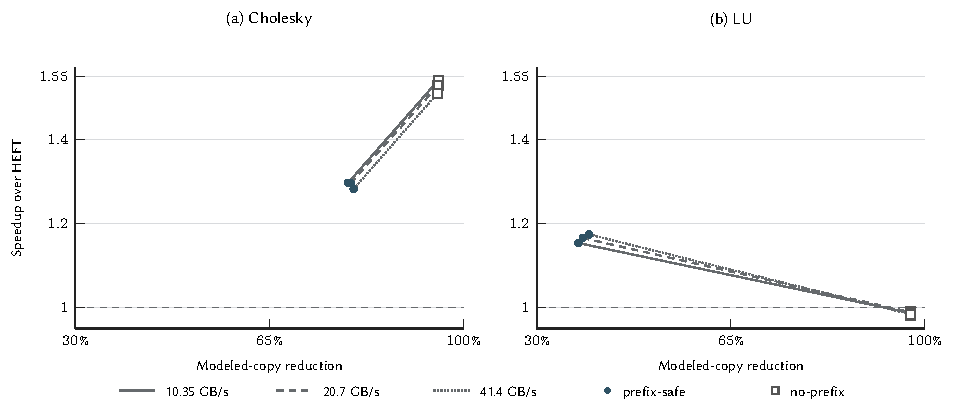
\includegraphics[width=0.97\textwidth]{figures/prefix_gate_ablation.pdf}
\Description{Prefix-safe versus exact gate removal at three scheduler copy-model bandwidths. Points are one-run diagnostics with no uncertainty estimate; dashed segments connect configurations that differ only in the prefix admission rule. LU exposes the protected-risk case, while Cholesky exposes the gate's conservative cost.}
\caption{Prefix-safe versus exact gate removal at three scheduler copy-model bandwidths. Dashed segments connect configurations differing only in prefix admission. Each point is a one-run diagnostic.}\label{fig:prefix-gate-sensitivity}
\end{figure*}

Across the three model values, Cholesky prefix-safe remains 1.282--1.296x faster than HEFT and no-prefix remains 1.509--1.540x faster. LU prefix-safe remains 1.153--1.173x faster, whereas no-prefix remains below HEFT at 0.983--0.989x. This qualitative persistence supports, but does not statistically establish, the mixed risk-control interpretation.

\subsection{Scheduler cost and excluded evidence}\label{negative-findings-determine-the-verdict}

In the primary matrix, four of fifteen workload--scheduler group medians meet our predeclared 5\% scheduler-share target and eleven miss it. All fifteen CG executions meet the target: median shares are 0.497\%, 0.377\%, and 0.375\% for H, P, and N. MiniWeather N has a 4.973\% median (3/5 repeats within target); MiniWeather P has a 5.079\% median (2/5 within). Every group median for FDTD, Cholesky, and LU is above target. In the historical 30-run block, all six group medians and all repeats miss: median shares for H, P, and N are respectively 13.47\%, 13.10\%, and 15.40\% on Cholesky and 10.87\%, 10.11\%, and 8.63\% on LU. Prefix-safe has lower absolute scheduler time and per-task cost than HEFT on both dense observations, but its shorter interval still leaves the ratio above target. The result is workload-dependent prototype cost, not universal incremental overhead caused by the prefix gate, and these measurements do not localize the cause.

An older source snapshot supplies secondary baseline and neutral-MiniWeather context, while a one-run compatibility bridge verifies deterministic comparator semantics. Their calibration and binaries differ from the clean experiment, so none of their timings are pooled or used as headline performance. Standard-CG performance from the historical same-path block is excluded because its identity control failed. We also exclude a dense-DAG transfer diagnostic whose raw logs were not archived and a MiniWeather SALC diagnostic without an emitted executed SHA.

Finally, a one-read--write/unique-owner restriction covers every task in the two dense observations and produces the same placements as the broad method. It therefore does not identify chains; prefix-safe remains a general locality refinement rather than a dense-DAG special case.

\section{Limitations and Threats to Validity}\label{limitations-and-threats-to-validity}

\textbf{Guarantee.} Prefix safety constrains only the modeled finish of placement decisions committed so far. SALC certifies one fixed-successor modeled inequality under a same-version/no-overwrite condition. Neither mechanism bounds an unscheduled suffix, proves global makespan improvement, or identifies a critical path.

\textbf{Problem coverage, selection, and arrival model.} The admission rule is defined independently of workload identity but addresses only prefix-admissible conflicts. The five-workload matrix distinguishes two effective modeled-copy-opportunity cases from three identical-placement controls; it estimates neither general conflict prevalence nor how often a conflict has enough frontier slack to be admissible. The two strongest configurations were selected after one-run exploration, so their repeated results establish behavior under observed opportunity rather than an unbiased frequency. The repeated DAGs are fully materialized before deferred submission. Decisions are still made one task at a time, but the evaluation does not validate dynamic task arrival, and the diagnostic fixed-successor case relies on graph-visible information. Results come from one 8-L4 node, one size per workload, and five repeats.

\textbf{Statistics and baselines.} The fixed H--P--N order can correlate direction with machine drift. FDTD's 1.064x P/H ratio under identical placement demonstrates that the effect is large enough to cross our materiality threshold. The 5/5 directions on the two different-placement cases, source-distinct replication, and exact gate-only code delta are descriptive evidence, not a randomized causal proof. The repeated evidence also lacks a strong weighted-copy or data-affinity baseline. We therefore claim improvement only over this runtime's HEFT-style selector and use no-prefix only to isolate the gate. Counterbalanced execution and repeated locality baselines are required to close this threat.

\textbf{Copy and memory model.} One 20.7 GB/s scalar and GPU-0 task-cost calibration are shared across identical L4s. The model omits pairwise NODE/SYS bandwidth differences, contention, overlap, memory capacity, and eviction. Modeled bytes/time are not physical PCIe traffic, and the results do not cover oversubscription or out-of-core execution.

\textbf{Traffic attribution.} Runtime-issued transfer accounting validates CUDASTF copy requests, not bus transactions. The controlled CG trace has no independent runtime version epoch, so its seven attributed requests are conditional on the task/data/fixed-successor join. CUPTI or equivalent profiling would be required for physical-link byte or time claims.

\textbf{Scheduler cost.} Eleven of fifteen primary group medians and all six historical group medians miss our predeclared share target, while CG demonstrates that the target can be met for all variants and repeats. The measurements do not isolate whether candidate evaluation, residency bookkeeping, task granularity, or other scheduler work dominates; lower-overhead implementation and broader validation remain future work.

\section{Related Work}\label{related-work}

\textbf{HEFT and bounded lookahead.} HEFT ranks a heterogeneous DAG and selects the processor that minimizes the current task's EFT, including communication that affects current input readiness \citep{topcuoglu2002heft}. PEFT augments this family with an optimistic future-cost table \citep{arabnejad2014peft}, while lookahead HEFT explicitly evaluates a placement's effect on child tasks \citep{bittencourt2010lookahead}. Anticipatory data-movement work similarly argues that future computation and I/O flows should inform movement decisions \citep{bleuse2018anticipation}. SALC is closest in spirit to one-hop lookahead, but its present certificate is narrower: one graph-visible fixed-device successor, runtime residency, and a HEFT-relative damage bound. Prefix-safe scheduling makes no successor prediction at all; it is a bounded online residual around the current HEFT choice.

\textbf{Task runtimes and locality-aware scheduling.} StarPU's early data-aware scheduler combined software-managed shared memory with transfer-aware placement \citep{augonnet2010dataaware,augonnet2011starpu}; PaRSEC \citep{bosilca2013parsec}, Legion \citep{bauer2012legion}, and CUDASTF \citep{nvidia2026cudastf} expose other abstractions for dependencies, placement, and data management. XKaapi's DADA scheduler uses data affinity \citep{bleuse2014dada}, LAHeteroprio studies how locality changes task-based performance \citep{bramas2019lahp}, and MCL uses locality-aware resource selection in a heterogeneous runtime \citep{kamatar2020locality}. Comparisons have also evaluated HEFT alongside data- and locality-aware multi-CPU/multi-GPU schedulers \citep{lima2015strategies}. Recent work formalizes locality scheduling under GPU-memory constraints \citep{gonthier2023taming}, and DARTS uses ready-task and bounded-future information for GPU/out-of-core linear algebra \citep{gonthier2025darts}. We therefore do not claim first data-aware scheduling. Our narrower contribution is an enforceable, time-shift-invariant admission gate around a HEFT-style per-task selector, paired with exact gate removal and explicit identity-placement controls.

\textbf{Transfer attribution.} HPCToolkit attributes GPU kernels and copies to heterogeneous calling contexts \citep{zhou2021hpctoolkit}. Our runtime-issued transfer stream serves a different diagnostic purpose: it joins scheduler decisions and logical-data identities to requested peer transfers. It does not replace a profiler and cannot establish physical PCIe transactions, overlap, or link time. The benchmark suite uses CUDASTF task graphs \citep{nvidia2026cudastf}; its sparse-CG path is related to the NAS CG kernel family \citep{bailey1991npb}, while MiniWeather adapts the public regional weather mini-app \citep{norman2020miniweather}.

\section{Conclusion}\label{conclusion}

A current-task EFT optimum can be a poor residency decision when a read--write placement moves the only valid version away from a future consumer. Prefix-safe copy-aware placement is a benchmark-independent admission rule for the prefix-admissible subclass of this conflict in CUDASTF's HEFT-style selector: it accepts lower-copy placements only within numerical tolerance of the current modeled-prefix finish bound and deliberately leaves other conflicts unchanged. In the qualified 75-run primary matrix, it reduces modeled copy and improves latency in all ten fixed-order pairs across the two different-placement cases. H, P, and N produce identical placement digests on the other three workloads; their timing differences bound scheduler-path and drift effects rather than supporting locality speedup or non-regression.

Exact gate removal exposes conservative cost on Cholesky, while prefix-safe beats no-prefix by 1.208x on LU despite no-prefix removing substantially more modeled copy and accumulating modeled-prefix damage. The result supports a condition-dependent risk control: the method is general, while the existence and profitability of a corrective deviation are properties of the observed task/residency state. A separate fixed-successor diagnostic conditionally eliminates seven attributed peer-copy requests and is followed by 27 downstream placement changes; it validates the constructed one-hop mechanism, not complete chain discovery or end-to-end causality.

Eleven of fifteen primary group medians miss our predeclared 5\% scheduler-share target, although all CG executions meet it. The present contribution is therefore an enforceable admission contract with condition-specific positive evidence and a prototype-level deployment limitation. Counterbalanced execution is the immediate evidential priority; broader systems and scales, independently selected conditions, dynamic arrival, stronger repeated locality baselines, physical transfer profiling, and lower scheduler cost are required before any universal performance claim.

\begin{acks}
OpenAI Codex assisted with adversarial manuscript review, experiment-protocol drafting, repository analysis, and language editing throughout Sections~1--9. The authors retain responsibility for the research design, source code, experimental execution, validation, and all claims~\citep{openai2026codex}.
\end{acks}

\section*{Artifact Availability}\label{artifact-pointers}

The implementation, harnesses, 75-run primary matrix, historical 30-run supporting block, raw qualified results, generated interpretation tables, and fail-closed verification scripts are prepared in source-locked artifacts. Primary and historical timings remain separate from instrumented forensic and provenance-incomplete diagnostics. A public immutable archive URL and final source tag will be inserted before submission.


\bibliographystyle{ACM-Reference-Format}
\bibliography{references}
% Absorb balance.sty's sub-baseline rounding on the short final page.
\par\kern2.4pt
\end{document}
